% 
%  EvaluationChapter.tex
%  ThesisISEL
%  
%  Created by Sana on 2023/08/09.
%

\chapter{Evaluation}
\label{cha:Evaluation_chapter}

The models were trained on the training datasets and their performance was evaluated with the validation dataset. This section describes experimental results obtained during the evaluation with validation set and other data from open-source projects. The chapter is also dedicated to discussing the results and comparing them to other related works in the field.

\section{Model Performance} % (fold)
\label{sec:Model_Performance}

A plot of the model evaluation was created, where the spread and the mean accuracy results of each model were compared. There is a population of accuracy measures for each algorithm because each algorithm was evaluated 10 times (via 10 fold-cross validation).

The data for the Command injection vulnerability was split into a 60\% training set and a 40\% test set, resulting in 7,872 samples for training and 5,248 for testing. The split was performed using the stratify method, which ensures that the proportion of target classes is preserved in both the training and testing sets. For the Null Pointer Dereference vulnerability, the data splitting process resulted in 1046 samples for training and 764 samples for testing.

Given our uncertainty about which algorithms and configurations would be suitable for our problem, we have created different models using the algorithms we previously mentioned.

\textbf{The training set} was used to train the selected models. It was where our models learns patterns and relationships within the data, and it served as the basis to choose the final model for the predictions.

During training, the model was exposed to the features (input data) and their corresponding target values (labels or output) from the training set. Model learning is carried out by adjusting its internal parameters based on the training data.

\textbf{The testing set} was used to evaluate the final model's performance on unseen data. It provided an estimate of how well our final model was likely to perform on new, real-world data.

Once the model was trained, it was evaluated on the testing set. The model's predictions were compared to the true target values, and performance metrics (e.g., accuracy, precision, recall) were calculated. This helped us in understanding how well the model generalized to data it hadn't seen before as we'll see next.


Before splitting the data, the \gls{smote} technique was applied, since we were having problem of class imbalance in dataset. This was done to ensure that the classes had approximately the same number of instances. This technique helped our model better learn and generalize from the data, resulting in improved classification performance.


\textbf{Note:} All tests, experiments, and evaluations presented in this section were conducted using the \gls{samate} data for the reasons explained earlier (Section \ref{sec:Data_Collection}). Despite the fact that we have used only \gls{samate} data, we were able to ensure that the results can be directly compared and provide a stable baseline for our analysis. The utilization of \gls{samate} data, with a sufficient number of examples, simplifies the assessment of the model's performance and enables clear comparisons between different configurations and techniques.

\newpage

\begin{table}[!ht]
    \centering
    \caption{Statistical summary of average performance among different probabilistic classifiers for Null Pointer Dereference.}
    \begin{tabular}{|l|l|l|}
    \hline
        \textbf{Vulnerability Type} & \multicolumn{2}{|c|}{\textbf{Null Pointer Deference}} \\ \hline
        Classification method &  mean accuracy & Standard deviation Accuracy \\ \hline
        Logistic regression & 0.996154 & 0.007692 \\ \hline
        Decision tree & 0.923385 & 0.024098 \\ \hline
        Support vector machines & 0.996154 & 0.007692 \\ \hline
        Naive Bayes & 0.996154 & 0.007692 \\ \hline
        Neighbor classifier & 0.996154 & 0.007692 \\ \hline
        Multi-layer Perceptron classifier & 0.999846 & 0.000462 \\ \hline
    \end{tabular}
	\label{tab:results_probabilistic_classifiers_NPD}
\end{table}

\begin{table}[!ht]
    \centering
    \caption{Statistical summary of average performance among different probabilistic classifiers for Command Injection.}
    \begin{tabular}{|l|l|l|}
    \hline
        \textbf{Vulnerability Type} & \multicolumn{2}{|c|}{\textbf{Command Injection}} \\ \hline
        Classification method &  Mean Accuracy & Standard deviation Accuracy \\ \hline
        Logistic regression & 0.998096 & 0.001528 \\ \hline
        Decision tree & 0.94919 & 0.008034 \\ \hline
        Support vector machines & 0.999873 & 0.000381 \\ \hline
        Naive Bayes & 0.999873 & 0.000381 \\ \hline
        Neighbor classifier & 0.999873 & 0.000381 \\ \hline
        Multi-layer Perceptron classifier & 0.999772 & 0.000684 \\ \hline
    \end{tabular}
	\label{tab:results_probabilistic_classifiers_CI}
\end{table}

Tables \ref{tab:results_probabilistic_classifiers_NPD}  and \ref{tab:results_probabilistic_classifiers_CI} show the results of the mean and standard deviation accuracy of the several probabilistic classifiers for Null Pointer Deference and Command Injection vulnerabilities.

\begin{figure}
  \centering
  \begin{subfigure}{\textwidth}
    \centering
    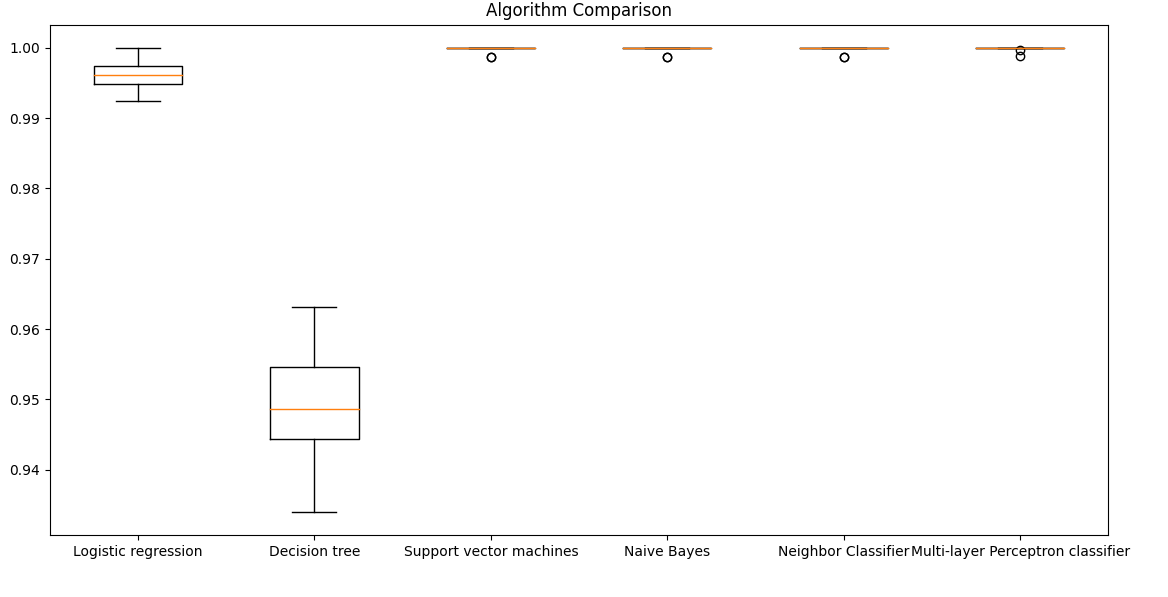
\includegraphics[width=\textwidth]{Plot_ML_CI}
    \caption{CI vulnerability}
    \label{fig:Plot_ML_CI_FIG}
  \end{subfigure}
  \hfill
  \begin{subfigure}{\textwidth}
    \centering
    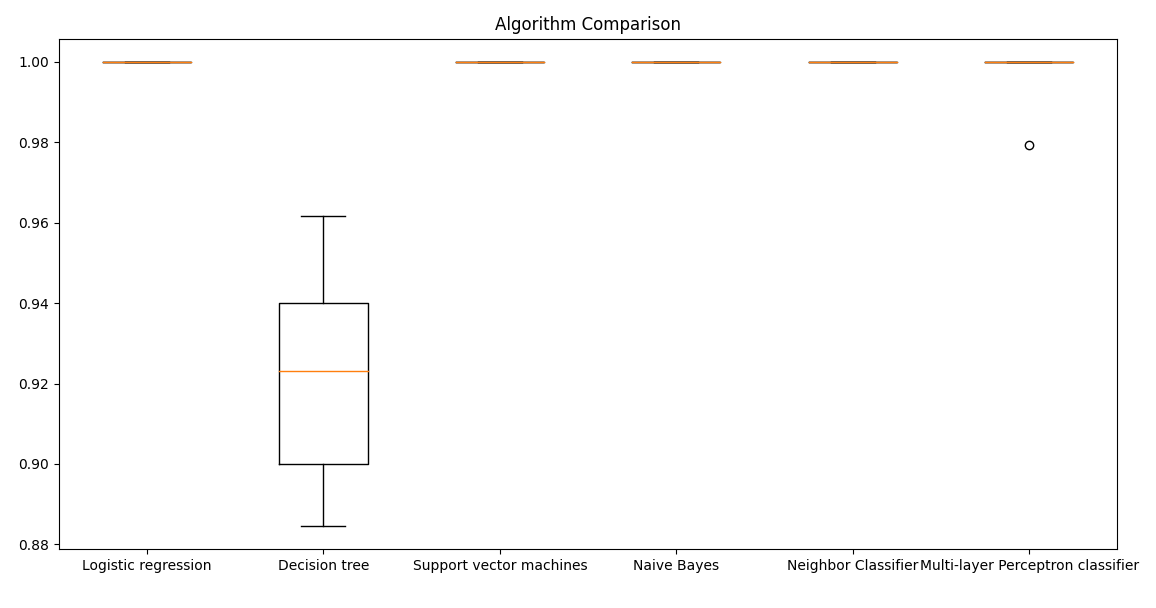
\includegraphics[width=\textwidth]{Plot_ML_NPD}
    \caption{NPD vulnerability}
     \label{fig:Plot_ML_CI_NPD}
  \end{subfigure}
  \caption{Box and Whisker Plot Comparing Machine Learning Algorithms for NPD and CI vulnerability}
   \label{fig:Plot_ML_BOX_FIG}
\end{figure}

Figures \ref{fig:Plot_ML_CI_FIG} and \ref{fig:Plot_ML_CI_NPD} show the box and whisker plots for each model, using the accuracy measure. Therefore, \gls{lr}, \gls{nb}, \gls{svm}, \gls{nc}, and \gls{mlpc} are the best algorithms for our dataset, as Figure \ref{fig:Plot_ML_BOX_FIG} illustrates. There are more options in choosing algorithms, which is beneficial for our model.

We can see in Figure \ref{fig:Plot_ML_BOX_FIG} that the box and whisker plots are squashed at the top of the range, with many evaluations achieving almost 100\% accuracy, and some pushing down into the high 90\% accuracy (in case of Decision Tree).

Given that there are several algorithms with good accuracy, we choose Logistic Regression to use in our final model. Next, the evaluation results obtained with the test set are presented for each type of vulnerability.

\newpage

\begin{figure}
  \centering

  \begin{subfigure}{0.7\textwidth}
    \centering
    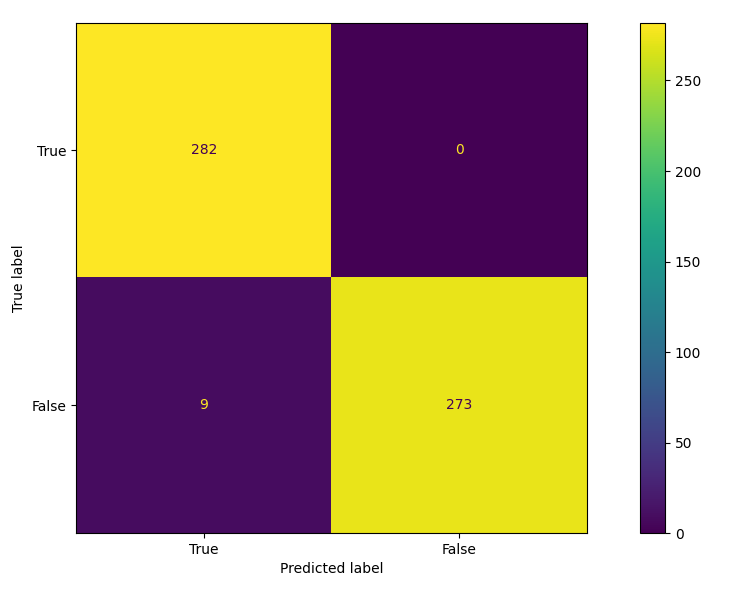
\includegraphics[width=\textwidth]{ConfusionMatrix_NPD2}
    \caption{NPD vulnerability}
    \label{fig:ConfusionMatrix_NPD_FIG}
  \end{subfigure}
  \hfill
  \begin{subfigure}{0.7\textwidth}
    \centering
    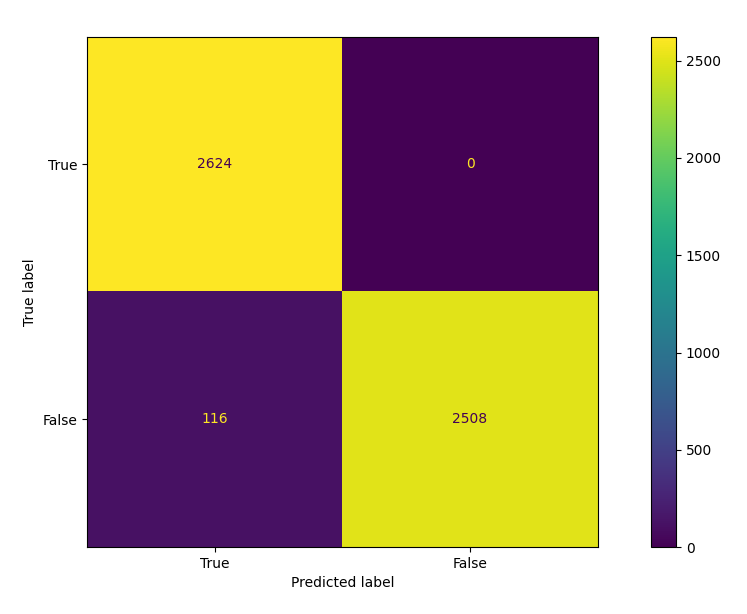
\includegraphics[width=\textwidth]{ConfusionMatrix_CI2}
    \caption{CI vulnerability}
    \label{fig:ConfusionMatrix_CI_FIG}
  \end{subfigure}

  \caption{Comparing LR model confusion matrix for NPD and CI vulnerability}
\end{figure}

Figures \ref{fig:ConfusionMatrix_NPD_FIG} and \ref{fig:ConfusionMatrix_CI_FIG} show the confusion matrix results for the LR models for both vulnerabilities, illustrating the true and predicted classifications for our test set.

\textbf{True Positive}: These are instances that were correctly predicted as vulnerable by the models. The models correctly identified 282 instances for \gls{npd} and 2624 for \gls{ci} as vulnerable.

\textbf{False Positive}: These are instances that were incorrectly predicted as vulnerable by the model. The model incorrectly identified 0 instances for \gls{npd} and 0 for \gls{ci} as vulnerable which is advantageous in our case.

\textbf{True Negative}: These are instances that were correctly predicted as not vulnerable by the model. The model correctly identified 273 instances for \gls{npd} and 2508 for \gls{ci} as not vulnerable.

\textbf{False Negative}: These are instances that were incorrectly predicted as not vulnerable by the model. The model missed 9 instances for \gls{npd} and 116 for \gls{ci} that were actually vulnerable.

\begin{figure}
     \begin{subfigure}[ht]{0.5\textwidth}
         \centering
         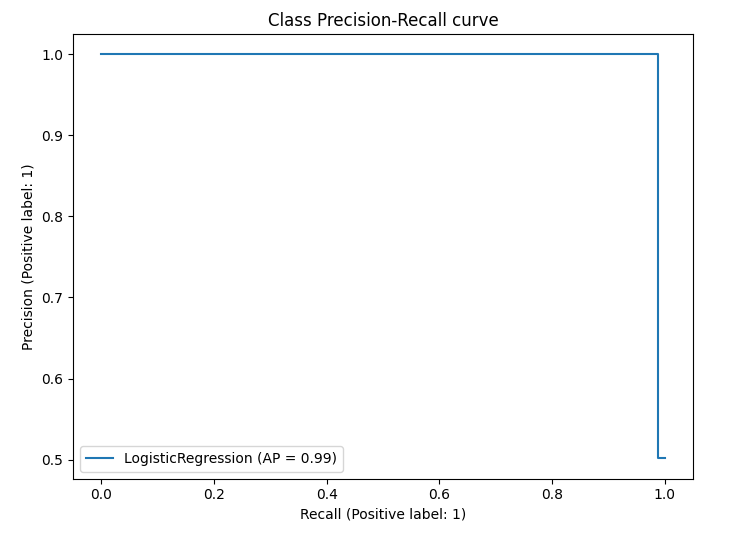
\includegraphics[width=\textwidth]{PrecisionRecall_NPD}
         \caption{\gls{npd} vulnerability}
         \label{fig:PrecisionRecall_NPD_FIG}
     \end{subfigure}
    \hfill
     \begin{subfigure}[ht]{0.5\textwidth}
         \centering
         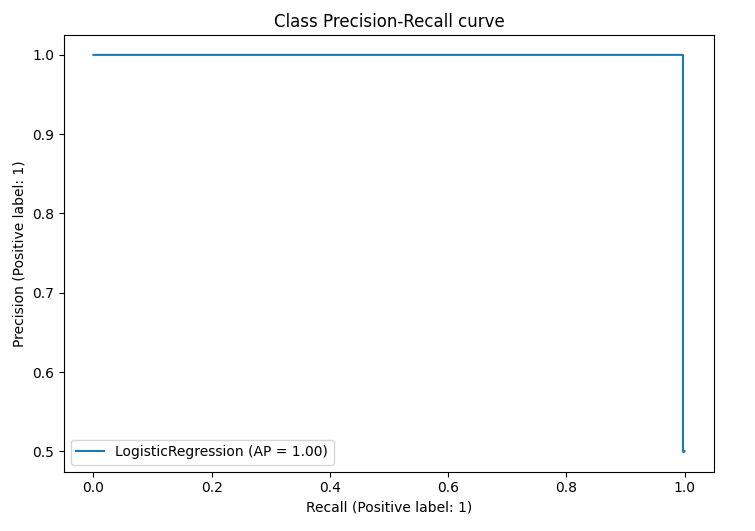
\includegraphics[width=\textwidth]{PrecisionRecall_CI}
         \caption{\gls{ci} vulnerability}
         \label{fig:PrecisionRecall_CI_FIG}
     \end{subfigure}
     \caption{LR model Precision-Recall Plot for \gls{npd} and \gls{ci} vulnerability}
     \hfill
\end{figure}

The precision-recall curve plot is represented in the Figures \ref{fig:PrecisionRecall_NPD_FIG} and \ref{fig:PrecisionRecall_CI_FIG} showing the precision/recall for each threshold for the logistic regression model. The graph represents recall on the x-axis and precision on the y-axis.

Once we have an Area Precision of 0.99, closer to 1, this means that the model has a good balance between precision and recall, effectively classifying well instances despite of false positives cases.

Figure \ref{fig:ClassificationReportCI_NPD_FIG} illustrates different classification metrics provided by scikit-learn tool's classification reports, detailing how well the model is performing on different classes.

\newpage

\begin{figure}
     \begin{subfigure}[ht]{0.5\textwidth}
         \centering
         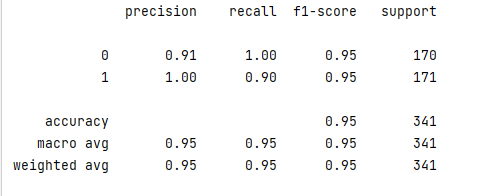
\includegraphics[width=\textwidth]{ClassificationReportNPD}
         \caption{\gls{npd} vulnerability}
         \label{fig:ClassificationReportNPD_FIG}
     \end{subfigure}
    \hfill
     \begin{subfigure}[ht]{0.5\textwidth}
         \centering
         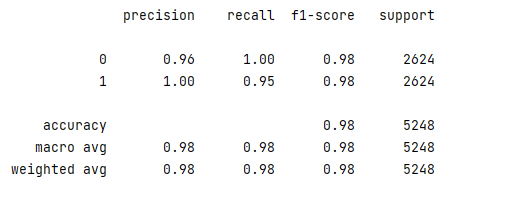
\includegraphics[width=\textwidth]{ClassificationReportCI}
         \caption{\gls{ci} vulnerability}
         \label{fig:ClassificationReportCI_FIG}
     \end{subfigure}
     \caption{Comparing LR classification report for \gls{npd} and \gls{ci} vulnerability}
     \label{fig:ClassificationReportCI_NPD_FIG}
     \hfill
\end{figure}

Figures \ref{fig:ClassificationReportNPD_FIG} and \ref{fig:ClassificationReportCI_FIG} show the classification report for different metrics such as precision, recall, F1-score, and support. The results show a high rate of these metrics for both vulnerable and not-vulnerable instances despite of false positive cases. 

\subsection{Discussion} % (fold)
\label{sec:Model_Creat_Eval_Discussion}

In this scenario, since a part of \gls{samate} data was also used to test the final model, we obtained good results. The models performed well for both vulnerabilities. There were a few cases of false negatives where the model failed to identify some functions that are actually vulnerable. 

We also have a good number of false positives, indicating that the model successfully identified all non-vulnerable functions. However, we will later discover that this number is just a false impression in the testing scenario with data from other projects. This is due to the fact that there are some functions that are supposedly not vulnerable but receive arguments with patterns identical to vulnerable functions.

It is necessary to further fine-tune the 'Var' attribute in order to match the pattern exactly (the same string if possible) with the truly vulnerable codes. This is because each project specifies values differently, which ended up being different from how it was specified in the \gls{samate} projects.

We have come to the conclusion that we have good models for both types of vulnerabilities with good performance, even with the cases of false positives, it was able to detect vulnerabilities in truly vulnerable places.


% section Model_Performance (end)


\section{Model Evaluation with data from other projects} % (fold)
\label{sec:Model_Eval_Other_Projects}

Given the good results with \gls{samate} data, we decided to analyse if our tool could detect vulnerabilities from real software projects.

We searched for some examples of vulnerable Java code on GitHub and found the following projects for Command injection vulnerability: Vulnerable Java Application \cite{github_Christophe}, Java Sec Code \cite{github_Syclover}, Operation System Command Injection Vulnerability in Java Spring \cite{github_Will}, Amaze File Manager \cite{github_Vishal}, OpenTSDB 2.4.0 Remote Code Execution \cite{github_Chris}, OS Command Injection \cite{github_Utku}, and the following projects for Null Pointer Deference vulnerability: null-pointer-dereference-examples \cite{github_Sridhar}, Selenium \cite{github_Harsha} and dbus-java \cite{github_David}.

For each project, we transformed the source code into dataset (feature extraction) with our dataset generator tool, by passing the project directory path to the tool, and then used the models trained with \gls{samate} data to find vulnerabilities. The output of our tool was a CSV file containing the file name, line number, node number and probability for each instance. We used manual inspection to confirm whether or not the projects are vulnerable. 

The results are resumed in Tables \ref{tab:model_evaluation_results_NPD} and \ref{tab:model_evaluation_results_CI}. The "Project" field indicates the name of the project. The "Vuln. Lines" indicates the number of vulnerable lines predicted by the model. The "Non-Vul. Lines" indicates the number of non-vulnerable lines predicted by the model. The "Tot. lines" indicates the total number of lines extracted from the project. The "Comments" provides a qualitative assessment of the model's behavior in that project. 

This qualitative assessment provides insights into the model's stability and generalization across different projects, even though we don't have ground truth labels for specific evaluation metrics.

\begin{table}[!ht]
    \centering
    \caption{Result of model evaluation  using real software projects for Null Pointer Deference vulnerability.}
    \begin{tabular}{|p{1.5in}|p{0.5in}|p{0.5in}|p{0.5in}|p{3in}|}
    \hline
        \textbf{Project} & \textbf{Vuln. Lines} & \textbf{Non-Vul Lines} & \textbf{Tot. lines } & \textbf{Comments} \\ \hline
        null-pointer-dereference & 25 & 160 & 185 & The model was able to detect the vulnerability, but the prediction was inconsistent. \\ \hline
        dbus-java & 38 & 238 & 276 & Incorrectly predicted. the prediction was inconsistent. \\ \hline
        SeleniumHQ & 70 & 1149 & 1219 & The model was able to detect vulnerable lines, but the prediction was inconsistent. \\ \hline
    \end{tabular}
	\label{tab:model_evaluation_results_NPD}
\end{table}

\newpage

\begin{table}[!ht]
    \centering
    \caption{Result of model evaluation  using real software projects for command injection vulnerability.}
    \begin{tabular}{|p{1.5in}|p{0.5in}|p{0.5in}|p{0.5in}|p{3in}|}
    \hline
        \textbf{Project} & \textbf{Vuln. Lines} & \textbf{Non-Vul Lines} & \textbf{Tot. lines } & \textbf{Comments} \\ \hline
        Vulnerable Java Application & 1 & 5 & 6 & Predicted correctly. The prediction was consistent. \\ \hline
        Java Sec Code & 20 & 218 & 238 & Incorrectly predicted. The prediction was inconsistent. \\ \hline
        OS Command Injection Vulnerability in Java Spring & 0 & 1 & 1 & In this project, it was only possible to extract one line to create the dataset, which is actually vulnerable. Unfortunately, the model missed it. The prediction was inconsistent. \\ \hline
        ArmazeFileManager & 116 & 1090 & 1206 & The model was able to detect the vulnerable functions. The prediction was inconsistent. \\ \hline
        OpenTSDB 2.4.0 Remote Code Execution & 220 & 2085 & 2305 & The model was able to detect the vulnerability, but the prediction was inconsistent. \\ \hline
        OS Command Injection & 0 & 3 & 3 & Incorrectly predicted. The prediction was inconsistent. \\ \hline
    \end{tabular}
	\label{tab:model_evaluation_results_CI}
\end{table}


As shown in the tables \ref{tab:model_evaluation_results_CI} and \ref{tab:model_evaluation_results_NPD} and explained earlier, the model is also detecting vulnerabilities (false positive cases) in functions that even though they receive variables whose values may come from input or null, and therefore tainted, are not actually vulnerable. Some of these functions don't even receive arguments, therefore, it doesn't make sense for them to be vulnerable.

\subsection{Discussion} % (fold)
\label{sec:Model_Eval_Discussion}

Based on this analysis, we can observe that in a significant number of projects, the models (for both type of vulnerabilities) predictions were inconsistent, meaning that they tend to be less stable (predicting some instances incorrectly). Nevertheless, it's worth noting that the models were successful in detecting vulnerabilities in certain projects.

We believe that the 'Var' feature requires further refinement to precisely match the pattern with the actual vulnerable code, ideally matching the same string. This is necessary because, as previously explained, each project specifies values in a different format than the \gls{samate} projects. Specifically, each project defines its own path for command execution, even when the commands themselves are identical. In other words, we think that the value of the 'Var' feature in the \gls{samate} dataset is different from the actual codes (due to each project being distinct), which is influencing significantly the vulnerability detection.


For \gls{ci} vulnerability: The source code contains file names and paths used in command execution, and these file-related details are considered as part of the model's input for detecting CI vulnerabilities.

For \gls{npd} vulnerability: the source code contains functions that receive variables as arguments. However, it's challenging to determine whether these variables are genuinely null through the static code analysis, especially when the variable serves as a parameter of a function. In other words, static code analysis cannot provide a straightforward way to identify null variables in the context of NPD vulnerabilities.

The structure of the 'var' attribute needs further refinement to ensure it is most suitable for the model, enabling the model to learn and make predictions effectively. Due to time constraints, this couldn't be done, and therefore, it remains for future work.

%%%%%%%%%%%%%%% Discussion %%%%%%%%%%%%%%%%%%%%%%%%%%%%%%%%%%%%%%%%%

\section{Comparison with other works} % (fold)
\label{sec:Comparison_with_other_works}

This section consists of comparisons with similar works in the field to provide a perspective from which observations and measurements are made for the evaluation of this work. As there are fundamental differences in each approach, direct comparison cannot be drawn between the outcomes. The results are summarized in Table \ref{tab:other_works_tab}. 

The current design of our tool is limited to Java programs. Future research should be conducted to adapt it for use with other programming languages.

The approaches are compared under the following aspects:
\begin{itemize}
\item \textbf{Scope and applicability}: has the model been trained on a single project and can it only classify files within that application, or is it generally applicable to any code from a large variety of sources;
\item \textbf{Programming language}: what programming language was subject of the study;
\item \textbf{Machine Learning Approach}: what machine learning approach was used;
\item \textbf{Vulnerability types}: which kinds of vulnerabilities can be detected;
\item \textbf{Dataset}: Is the data sourced from real-world projects or from synthetic databases, such as \gls{samate} data.
\end{itemize}

%\begin{table}[!ht]
%    \centering
%    \caption{Results of comparisons with similar works}
%    \begin{tabular}{|p{1in}|p{0.5in}|p{1in}|p{0.9in}|p{1in}|p{0.4in}|p{0.4in}|p{0.4in}|}
%    \hline
%        \multicolumn{5}{|c|}{\textbf{Aspects of the approach}} &  \multicolumn{3}{|c|}{\textbf{Result. Metrics}} \\ \hline
%        \textbf{Tool Name} & \textbf{Prog. Lang.} & \textbf{Vul. Type} & \textbf{Scope \& applicability} & \textbf{Mach. Learn. Approach} & \textbf{Acc.} & \textbf{Prec.} & \textbf{F1-Score} \\ \hline
%        SWD-SCA-ML (our tool) & Java & CI, NPD & General & Supv. Learn., Prob. Classifiers & 96.5\% & 95\% & 96.5\% \\ \hline
 %       WIRECAML & PHP & SQLi, XSS & Incl. & Supv. Learn., Prob. Classifiers & 95\% & 94\% & 94\% \\ \hline
%        VUDENC & Python & SQLi, XSS, CI, XSRF & General & Supv. Learn., Deep Learn. & 97\% & 91\% & 87\% \\ \hline
%        VulDeePecker & C/C++ & buffer error, resource management error & General & Supv. Learn., Deep Learn. & 87\% & 88.1\% & 95\% \\ \hline
%    \end{tabular}
%    \label{tab:other_works_tab}
%\end{table}

\begin{table}[!ht]
    \centering
    \caption{Results of comparisons with similar works}
    \begin{tabular}
    %{\textwidth}{|X|X|X|X|X|X|}
    {|p{1in}|p{0.5in}|p{1in}|p{0.9in}|p{1in}|p{1in}|}
    \hline
        \multicolumn{6}{|c|}{\textbf{Aspects of the approach}} \\ \hline
        \textbf{Tool Name} & \textbf{Prog. Lang.} & \textbf{Vul. Type} & \textbf{Scope \& applicability} & \textbf{Mach. Learn. Approach} & \textbf{Dataset} \\ \hline
        SWD-SCA-ML (our tool) & Java & CI, NPD & General & Supv. Learn., Prob. Classifiers & Real \& Synth. \\ \hline
        WIRECAML & PHP & SQLi, XSS & Inconclusive & Supv. Learn., Prob. Classifiers & Real \& Synth. \\ \hline
        VUDENC & Python & SQLi, XSS, CI, XSRF & General & Supv. Learn., Deep Learn. & Real \& Synth. \\ \hline
        VulDeePecker & C/C++ & resource management error, buffer error & General & Supv. Learn., Deep Learn. & Real \& Synth. \\ \hline
    \end{tabular}
    \label{tab:other_works_tab}
\end{table}

\subsection{Discovering vulnerabilities using data-flow analysis and machine learning} % (fold)
\label{sub:related_work1}

This is the main work related to our problem, proposed by Kronjee et al. \cite{Kronjee2018}. It combines static code analysis with machine learning for detecting SQL injection (SQLi) and Cross-Site Scripting (XSS) vulnerabilities in PHP applications. It also uses SAMATE for collecting training data for the model \cite{Kronjee2018}.

The work attempted to contribute and demonstrate that it is possible to combine machine learning with static code analysis for detecting vulnerabilities in software. However, we suggest that the demonstrated results show some uncertain, especially when testing the tool with different data (data from other applications). This is because they did not demonstrate the data extracted from other applications. In other words, their work did not include a demonstration of the data extracted from other applications, which was used to test their tool. Furthermore, based on our analyses, we suggest that their process for feature extraction and dataset creation is based on a method that does not consistently define features according to the function names and variable number of features. The features extracted from the source codes are functions (function names), which can differ from project to project, and the size of features could also vary from project to project. In this sense, the work may not be considered definitive, as it could be challenging to apply the model created and trained with a specific dataset (e.g., SAMATE data) to any other dataset extracted from a different project or source code.

The authors built a tool called WIRECAML \cite{Kronjee2018} and Table \ref{tab:kronj_res_tab} presents the results of WIRECAML using various classifiers trained on SAMATE and NVD data. We have made comparisons regarding the accuracy of their model with ours for some classifiers that we have used in common, since it's not possible to make a comparison regarding the types of vulnerabilities used in both cases.

The main advantage of our tool over theirs is its versatility. In our case, our model can be applied to any dataset generated using our tool. On the other hand, in their case, it remains inconclusive whether their model can be applied to any dataset generated by their tool, due to the features that they have considered as previously explained in the preceding paragraph.

\begin{table}[!ht]
    \centering
    \caption{Comparison of several probabilistic classifiers in terms of AUC-PR values extracted from \cite{Kronjee2018}}
    \begin{tabular}{|l|l|l|}
    \hline
        \textbf{Classification method} & \textbf{Vulnerability} & \textbf{AUC-PR} \\ \hline
        Decision tree & SQLi & 0.88 \\ \hline
        Random forest & SQLi & 0.85 \\ \hline
        Logistic regression & SQLi & 0.87 \\ \hline
        Naive Bayes & SQLi & 0.64 \\ \hline
        TAN & SQLi & 0.75 \\ \hline
        Decision tree & XSS & 0.82 \\ \hline
        Random forest & XSS & 0.82 \\ \hline
        Logistic regression & XSS & 0.79 \\ \hline
        Naive Bayes & XSS & 0.69 \\ \hline
        TAN & XSS & 0.81 \\ \hline
    \end{tabular}
    \label{tab:kronj_res_tab}
\end{table}


%\begin{figure}[ht]	
%	\centering
%	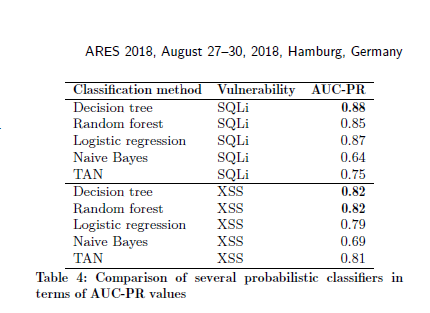
\includegraphics[width=0.90\textwidth]{Result_WIRECAML.}
%	  \caption{Model evaluation result obtained by the WIRECAML tool.}
%  \label{fig:bibtex}
%\end{figure}

Our model achieved better results when using the same classifiers compared to their model. Their work has limitations in feature extraction for dataset construction, and this represents the primary advantage of our work over theirs. The model created by our tool can be applied to datasets extracted from other applications since it considers the same features.



% subsection related_work1(end)

\subsection{VUDENC - Vulnerability Detection with Deep Learning on a Natural Codebase} % (fold)
\label{sub:related_work_vudenc}

It is a vulnerability detection system that utilizes neural networks to learn vulnerable features from a collection of data extracted from GitHub. The work focuses on the Python programming language and exclusively learns source code \cite{Wartschinski2019}. 

This work managed to demonstrate the potential use of deep learning directly on source code to learn vulnerable features, utilizing LSTM (Long Short-term Memory) models \cite{article_LSTM}.

They created the model using LSTM and managed to achieve good results. With an F1 score of around 87\%, they attained a precision of 91\% and a recall of 83\%.

Their tool was able to detect several types of vulnerabilities, and this is the main advantage of their work compared to ours. Another advantage in comparison with our approach is that they used real GitHub data for model creation. In our case, we used SAMATE data for training and model creation.



% subsection related_work_vudenc(end)

\subsection{VulDeePecker Deep Learning Based System For Vulnerability Detection} % (fold)
\label{sub:related_work_VulDeePeckerADeep}

Li et al. \cite{Zhen_Li2018} developed this tool  to detect buffer error vulnerabilities and resource management error vulnerabilities in C/C++ programs. They work on a "code gadget database" made from a large number of popular open source projects, including the Linux kernel and Firefox. The vulnerabilities are found by using the NVD and SAMATE dataset, which contain synthetic and real-life / production code, flaws, and vulnerabilities.

Selecting their data from those sources, Li et al work on very high-quality code. Similar to our approach, they also collected projects with vulnerable source code to extract their own features and create the dataset. They labeled all vulnerable locations in source codes, just as we did, but they did so manually. This differs from our approach, which automates this entire process.

They train a bidirectional LSTM and achieve an impressive F1 score of around 85-95\%. Our tool achieve quite the same high score too. Furthermore, their database only consists of synthetic code as well.

The authors of VulDeePecker compared their tool to other approaches and found a precision of 25\% for the Flawfinder  tool \cite{Flawfinder_}, 39.6\% for Checkmarx \cite{Checkmarx_}, and 19.4\% for RATS \cite{RATS_}, in contrast to VulDeePecker's precision of 88.1\%. Which means that VulDeePecker is more effective than these tools. The VulDeePecker approach successfully was able to reduce the number of false positive results to almost zero, a level of achievement that we were unable to accomplish in our case.

% subsection related_work_VulDeePeckerADeep(end)

% section Comparison_with_other_works (end)

\section{Limitations} % (fold)
\label{sec:LIMITATIONS_SEC}

The present design, implementation, and evaluation of this work have several limitations, which suggest interesting open problems for future research. First, the present design of this work is limited to deal with a variety of different types of vulnerabilities. The feature extraction process is a challenging problem for projects compatibilities with Java programming language version 8, as well as with higher versions due to the functional programming paradigms (dealing with lambda expressions on features extraction).

Second, the present design of our tool only deals with Java programs. Future research needs to be conducted to adapt it to deal with other kinds of programming languages.

Third, the present design of this work only deals with vulnerabilities related to functions invocation. The future work could investigate how to detect the other kinds of vulnerabilities by leveraging the other kinds of key points.

Fourth, The data collected for model creation was just from one source (SAMATE) and  insufficient, it's necessary to collect more data from different sources and from real example source code.

Fifth, the evaluation of the model's performance was conducted using standard measures commonly used in the context of vulnerability prediction, such as predictions, accuracy, precision, and recall. By using these well-established metrics, the study aimed to minimize potential risks to the validity of its conclusions. However, in practice, there may be other metrics and representation demonstrating how well a classifier performs. In essence, the evaluation process used common and accepted measures but we acknowledge the possibility of further metrics that might be valuable for assessing classifier performance.

Sixth, our current tool implementation is limited to the use of machine learning classifiers. To enhance our systematic experiments, we can explore alternative learning techniques for vulnerability detection, including Natural Language Processing, Recurrent Neural Networks, and Convolutional Neural Networks (CNNs). It's also possible to combine these methods for a more comprehensive and holistic approach.

Seventh, the present  method of model creation is limited because the hyperparameter tuning process was not used. It can be a crucial step in model creation to tune parameters in machine learning in order to adjusting the settings of a machine learning algorithm or model to ensure that the model performs at its best.

Finally, furthermore, design decisions were made which might affect the overall end result.


% section LIMITATIONS_SEC (end)


% section Model_Eval_Other_Projects (end)